\documentclass{article}
\usepackage{amsmath} %This allows me to use the align functionality.
                   %If you find yourself trying to replicate
                   %something you found online, ensure you're
                   %loading the necessary packages!
\usepackage{amsfonts}%Math font
\usepackage{graphicx}%For including graphics
\usepackage{hyperref}%For Hyperlinks
\usepackage{natbib}        %For the bibliography
\bibliographystyle{apalike}%For the bibliography
\usepackage[margin=1.0in]{geometry}
\usepackage{float}
\usepackage{Sweave}
\begin{document}
\Sconcordance{concordance:HW2.tex:HW2.Rnw:%
1 12 1 1 0 99 1 1 6 8 0 1 2 18 1 1 12 11 0 1 2 1 3 33 0 1 3 7 1 1 7 6 0 %
1 3 22 0 1 2 5 1 1 7 6 0 1 7 9 0 1 3 1 2 1 0 2 1 1 10 9 0 1 3 6 0 1 2 9 %
1 1 3 2 0 2 1 1 7 9 0 1 2 7 1 1 3 8 0 1 2 2 1 1 2 10 0 1 3 50 1 1 5 7 0 %
1 6 7 0 1 6 7 0 1 6 7 0 1 2 22 1 1 3 2 0 6 1 1 17 19 0 1 2 1 1 1 68 1 2 %
1 3 2 0 6 1 1 17 19 0 1 2 2 1 1 68 1 2 1 3 2 0 6 1 1 17 19 0 1 2 2 1 1 %
68 1 2 1 3 2 0 6 1 1 17 19 0 1 2 2 1 1 68 1 2 2 1 9 0 1 8 1 1 1 3 2 0 1 %
3 5 0 1 2 1 3 2 0 1 3 5 0 1 2 1 3 2 0 1 3 5 0 1 2 21 1 1 2 1 0 1 2 1 0 %
1 7 10 0 1 2 4 1 1 2 1 0 3 1 1 9 12 0 1 2 7 1 1 2 1 0 3 1 1 2 2 1 1 13 %
16 0 1 3 8 1 1 3 2 0 1 1 6 0 1 2 4 1 1 4 3 0 1 2 1 0 1 1 6 0 1 2 4 1 1 %
3 8 0 1 2 4 1 1 4 9 0 1 2 6 1 1 3 8 0 1 2 4 1 1 4 3 0 1 2 1 0 1 1 6 0 1 %
2 4 1 1 4 3 0 1 2 1 0 1 1 6 0 1 2 17 1 1 3 2 0 1 1 17 0 1 2 63 1 1 3 2 %
0 1 1 3 0 1 2 18 1 1 2 6 0 1 1 6 0 1 2 4 1 1 3 2 0 1 2 16 0 1 2 4 1 1 2 %
6 0 1 2 7 0 1 2 7 1 1 2 1 0 1 5 7 0 2 2 1 0 4 1 1 2 1 1 3 0 1 2 1 3 2 0 %
3 1 1 12 15 0 1 2 3 1 1 2 1 0 1 1 3 0 1 2 19 1 1 3 2 0 2 1 1 2 14 0 1 4 %
2 0 1 1 14 0 1 2 2 1 5 0 2 1 3 0 1 2 1 3 2 0 3 1 1 13 16 0 1 2 5 1 1 2 %
1 0 2 1 1 2 1 1 1 2 2 1 1 2 1 1 1 2 1 0 1 2 1 0 1 1 3 0 1 2 10 1}

%set the size of the graphs to fit nicely on a 8.5x11 sheet
\noindent \textbf{MA 354: Data Analysis I -- Fall 2019}\\%\\ gives you a new line
\noindent \textbf{Homework 2:}\vspace{1em}\\
\emph{Complete the following opportunities to use what we've talked about in class. 
These questions will be graded for correctness, communication and succinctness. Ensure
you show your work and explain your logic in a legible and refined submission.}\\
%Comments -- anything after % is not put into the PDF

\begin{enumerate}
%%%%%%%%%%%%%%%%%%%%%%%%%%%%%%%%%%%%%%%%%%%%%%%%%%%%%%%%%%%%%%%%%%%%%%%%%%%%%%%
%%%%%%%%%%%%%%%%%%%%%%%%%%%%%%%%%%%%%%%%%%%%%%%%%%%%%%%%%%%%%%%%%%%%%%%%%%%%%%%
%%%%%%%%%  Question 0
%%%%%%%%%%%%%%%%%%%%%%%%%%%%%%%%%%%%%%%%%%%%%%%%%%%%%%%%%%%%%%%%%%%%%%%%%%%%%%%
%%%%%%%%%%%%%%%%%%%%%%%%%%%%%%%%%%%%%%%%%%%%%%%%%%%%%%%%%%%%%%%%%%%%%%%%%%%%%%%
\item[0.] \textbf{Complete weekly diagnostics.}

%%%%%%%%%%%%%%%%%%%%%%%%%%%%%%%%%%%%%%%%%%%%%%%%%%%%%%%%%%%%%%%%%%%%%%%%%%%%%%%
%%%%%%%%%%%%%%%%%%%%%%%%%%%%%%%%%%%%%%%%%%%%%%%%%%%%%%%%%%%%%%%%%%%%%%%%%%%%%%%
%%%%%%%%%  Question 1
%%%%%%%%%%%%%%%%%%%%%%%%%%%%%%%%%%%%%%%%%%%%%%%%%%%%%%%%%%%%%%%%%%%%%%%%%%%%%%%
%%%%%%%%%%%%%%%%%%%%%%%%%%%%%%%%%%%%%%%%%%%%%%%%%%%%%%%%%%%%%%%%%%%%%%%%%%%%%%%
\item  The goal of this question is to ensure you can simply explain it to yourself in preparation
for the next exam and final. Think of this as an opportunity to make something 
quick you can read that summarizes all of our discussions about this topic
that you can study from later.

\textbf{(Part A)} Succinctly describe what a probability model tells us. Your solution should
discuss PMF, PDF, and CDF.
\newline
\newline
\textbf{Solution:}
The distribution of a variable tells us what values the variable takes and how often it takes these values. A probability model is rooted in the distribution of a variable and tells us how likely an event is to occur. 
PMF is the probability mass function for discrete variables and represents the probability that discrete random variable X takes some value x. Mathematically, this is P(X=x). 
PDF is the probability density function and characterizes the probability of a continuous random variables. P(X=x) for a PDF is zero because it deals with continuous data, therefore the PDF defines the probability curve. 
CDF is the cumulative distribution function of a random variable for discrete and continuous data. It gives the probability that random variable X is less than or equal to some value x, represented mathematically as P(X<=x).
\newline

\textbf{(Part B)} Succinctly describe what $E(X)$ and $var(X)$ tell us.
\newline
\newline
\textbf{Solution:}
$E(X)$ tells us the expected value, or population parameter for some random variable X. 
$var(x)$ tells us the expected variance of some population parameter for some random variable X. 
\newline

\textbf{(Part C)} Describe the process of finding a method of moments estimator.
\newline
\newline
\textbf{Solution:}
A method of moments estimator estimates values for parameters that define a distribution by using moments from a sample distribution. It is quicker and easier than the MLE and works best with large n. Generally, it uses moments (expected value and variance) from a sample data set and sets them equal to the population moments and solves the system of equations to derive the parametersof interest.
\begin{enumerate}
  \item For a distribution with one parameter
  \newline
    1. Set E(X) = sample mean and solve for the parameter
    \newline
    2. Solve for the parameter
  \item For a distribution with two parameters.
  \newline
    1. Set E(X) = sample mean
    \newline
    2. Set var(x) = sample variance
    \newline
    3. Solve for the parameters
\end{enumerate}

\textbf{(Part D)} Succinctly describe the process of finding a maximum likelihood estimator.
\newline
\newline
\textbf{Solution:}
The MLE tries to figure out what combination of parameters makes the given, fixed sample data most likely. It assumes some distribution that characterizes the distribution is true and estimates the parameter that maximizes the likelihood of observing the sample distribution. It systematically underestimates the parameter but will always output a value within the range of data. 
\newline

%apologies for my not succinct answer
%I just wanted to make sure I had a good understanding of CLT before moving forward
\textbf{(Part E)} Succinctly describe what CLT tells us.
\newline
\newline
\textbf{Solution:}
The central limit theorem tells us the sampling distribution for certain estimators. 
\newline
\newline
CLT 1 applies to a random sample from a Gaussian distribution. The sample parameter is Gaussian distributed where the expected value of the population parameter is equal to the value of the sample parameter and the standard error is equal to the radical of the quantity of the population variance divided by n, the sample size. As the sample size increases, the estimation of the population parameter varies less. There is no sample size requirement for CLT 1.
\newline
\newline
CLT 2 applies to a random sample of nonnormal data. This version of the theorem says that if the populatioin standard deviation is known, the sample averages will be approximately Gaussian distributed even if the underlying population distribution is not. This requires that n is greater than or equal to 30. As the sample size increases, the quality of approximation increases and the variation of the sample mean decreases. When we standardize the sample mean using Z, the centered and scaled version of the sample mean, the data is then Gaussian distributed. 
\newline
\newline
CLT 3 takes nonnormal data with an unknown population standard deviation and n greater than or equal to 30. The sample mean is approximately Gaussian distributed and when we standardize the sample mean, the data is approximately Gaussian. If we replace the population variance with the known sample variance in the Z standardization, the sample distribution is approximately t distributed. Again, the sampling distribution approximation holds, even if the underlying population distribution is not perfectly Gaussian.
CLT 4 takes a random sample of Bernoulli data. The population mean is set equal to the population proportion and the variance of the population mean is equal to the population proportion multiplied by 1 minus the population proportion. The distribution of the sample proportion is approximately Gaussian. The sample proportion is equal to the sample mean because the sample proportion measures the probability of success in the sample. Since the sample is Bernoulli data, when the sum of the successes (which all take the value of 1) is divided by the sample size or number of observations, this calculates the mean mathematically, giving the value of x bar but also the probability of success. 
\newpage
%%%%%%%%%%%%%%%%%%%%%%%%%%%%%%%%%%%%%%%%%%%%%%%%%%%%%%%%%%%%%%%%%%%%%%%%%%%%%%%
%%%%%%%%%%%%%%%%%%%%%%%%%%%%%%%%%%%%%%%%%%%%%%%%%%%%%%%%%%%%%%%%%%%%%%%%%%%%%%%
%%%%%%%%%  Question 2
%%%%%%%%%%%%%%%%%%%%%%%%%%%%%%%%%%%%%%%%%%%%%%%%%%%%%%%%%%%%%%%%%%%%%%%%%%%%%%%
%%%%%%%%%%%%%%%%%%%%%%%%%%%%%%%%%%%%%%%%%%%%%%%%%%%%%%%%%%%%%%%%%%%%%%%%%%%%%%%
\item \textbf{(Point Estimation)} Consider Example 7.4 in the notes.
The following data represents battery lifetimes measured in hours 
for $n=50$ batteries.
\begin{Schunk}
\begin{Sinput}
> dat.battery<-c(4285,2066,2584,1009,318,1429,981,1402,1137,414,
+        564, 604, 14, 4152, 737, 852, 1560, 1786, 520, 396,
+        1278,209, 349, 478, 3032, 1461, 701, 1406, 261, 83,
+        205, 602, 3770, 726, 3894, 2662, 497, 35, 2778, 1379,
+        3920, 1379, 99, 510, 582, 308, 3367, 99, 373, 4540)
\end{Sinput}
\end{Schunk}
In the notes, we modeled this data with the exponential distribution. For this exercise, let's
consider the \textbf{Weibull distribution}, which is used to model device failure rates.
The flexibility of the Weibull distribution allows engineers to model constant failure rates as 
well as increasing or decreasing rates.
\begin{align*}
\beta, \eta &\in \mathbb{R}^+ \tag*{\textbf{[Parameters]}}\\
\mathcal{X}&= \{\omega: \omega \in (0,\infty)\} \tag*{\textbf{[Support]}}\\
f_X(x|\beta,\eta) &= \frac{\beta}{\eta} \left(\frac{x}{\eta}\right)^{\beta-1} e^{-\left(\frac{x}{\eta}\right)^\beta}~ I(x \in (0,\infty)) \tag*{\textbf{[PDF]}}\\
F_X(x|\beta,\eta) &=  \left[1- e^{-\left(\frac{x}{\eta}\right)^\beta}\right]I(x>0)\tag*{\textbf{[CDF]}}\\
F_X^{-1}(p|\lambda)&=\eta \left(-\log(1-p)\right)^{\frac{1}{\beta}}\tag*{\textbf{[For $p \in (0,1)$]}}\\
E(X) &= \eta \Gamma\left( 1+ \frac{1}{\beta}\right)\tag*{\textbf{[Expected Value]}}\\
var(X) &= \eta^2 \left[\Gamma\left( 1+ \frac{2}{\beta}\right)-\left(\Gamma\left( 1+ \frac{1}{\beta}\right)\right)\right]^2 \tag*{\textbf{[Variance]}}\\
\end{align*}
\textbf{Hint:} The function $\Gamma(\cdot)$ can be calculated using \texttt{gamma()} in \texttt{R}.
\begin{enumerate}
  \item \textbf{Solve for the method of moments estimates for $\beta$ and $\eta$.}
  \newline
  \textbf{Solution:}
  \newline
\begin{Schunk}
\begin{Sinput}
> #method of moments
> g<-function(x.data,theta) {#data, theta
+   #set the sample and population mean equal
+   beta = theta[1]
+   nu = theta[2]
+   EX = nu*gamma(1+(1/beta))
+   varX = (nu^2)*(gamma(1+(2/beta))-(gamma(1+(1/beta)))^2)
+   m1 = EX - mean(x.data)
+   m2 = varX - var(x.data)
+   return(c(m1,m2))
+ } 
> library(nleqslv) #load 
> nleqslv(x=c(1,1000), #best guess
+         fn=g, #function
+         x.data=dat.battery)
\end{Sinput}
\begin{Soutput}
$x
[1]    1.039419 1377.130555

$fvec
[1] 1.100943e-09 2.366095e-05

$termcd
[1] 2

$message
[1] "x-values within tolerance 'xtol'"

$scalex
[1] 1 1

$nfcnt
[1] 9

$njcnt
[1] 1

$iter
[1] 9
\end{Soutput}
\begin{Sinput}
> 
\end{Sinput}
\end{Schunk}
\citep{nleqslv}
\newline
Using the method of moments estimation technique, we found that the values for beta and eta were 1.039419 and 1377.130555, respectively. Beta represents the "shape" parameter, or the expected value for the weibull distribution and eta represents the "scale" parameter, or the variance. Method of moments estimation solves for the value of these two parameters by setting the sample expected value and variance equal to the population value and variance and solving. Using the nleqslv package with our best guesses being a vector from 1 to 1000, given the recommendation from the moodle board, we received our estimates as stated before. It is interesting to note that when I originally put my best guess as 0 to 1000, it produced an error. This must be because when solving for the values, we take a root, which requires positive values. 
\newline
  \item \textbf{Solve for the maximum likelihood estimates for $\beta$ and $\eta$.}
  \newline
  \textbf{Solution:}
  \newline
\begin{Schunk}
\begin{Sinput}
> #Maximum Likelihood Estimation
> weibull.ll<-function(x.data,theta){ #data, theta
+   beta <- theta[1]
+   nu <- theta[2]
+   return(-1*sum(dweibull(x.data, shape=beta, scale=nu, log = TRUE)))
+ }
> optim(fn = weibull.ll, #function
+       par = c(1,5000), #best guess
+       x.data = dat.battery) #data
\end{Sinput}
\begin{Soutput}
$par
[1]    1.003204 1357.910932

$value
[1] 410.6091

$counts
function gradient 
      91       NA 

$convergence
[1] 0

$message
NULL
\end{Soutput}
\end{Schunk}
The maximum likelihood estimates for beta and eta are 1.003204 and 1357.910932, respectively. These estimates are similar, but different from the MOM estimates.
\newline
  \item \textbf{Plot a histogram of the data with the estimated Weibull distributions superimposed.}
  \newline
  \textbf{Solution:}
  \newline
\begin{Schunk}
\begin{Sinput}
> #MOM distribution
> mom.weibull<-data.frame(x=c(0:5000), 
+                         f=dweibull(x=c(0:5000), 
+                         shape= 1.039419,#from nleqslv
+                         scale = 1377.130555, #from nleqslv
+                         log=FALSE))
> #MLE distribution
> mle.weibull<-data.frame(x=c(0:5000), 
+                         f=dweibull(x=c(0:5000), 
+                         shape=1.003027, #from ll fn
+                         scale = 1357.504746, #from ll fn
+                         log=FALSE))
> 
\end{Sinput}
\end{Schunk}

\begin{Schunk}
\begin{Sinput}
> library(ggplot2) #load ggplot
> library(gridExtra) #load gridarrange
> ggdat<-data.frame(lifetime=dat.battery)
> g1<-ggplot(data=ggdat, aes(x=lifetime))+
+   geom_histogram(aes(y=..density..),color="black",fill="lightblue", bins=15)+
+   geom_hline(yintercept=0)+
+   theme_bw()+
+   xlab("Battery Lifetime (in hours)")+
+   ylab("Density")+
+   ggtitle("Battery Lifetime Data fitted with Weibull Distributions", 
+           subtitle = "Using MOM and MLE Estimates")+
+   geom_line(data=mom.weibull, aes(x=x, y=f, color="MOM"))+
+   geom_line(data=mle.weibull, aes(x=x,y=f, color="MLE"))
>                  #linetype="dotted", 
>                  #alpha = 0.05)
> g1
\end{Sinput}
\end{Schunk}
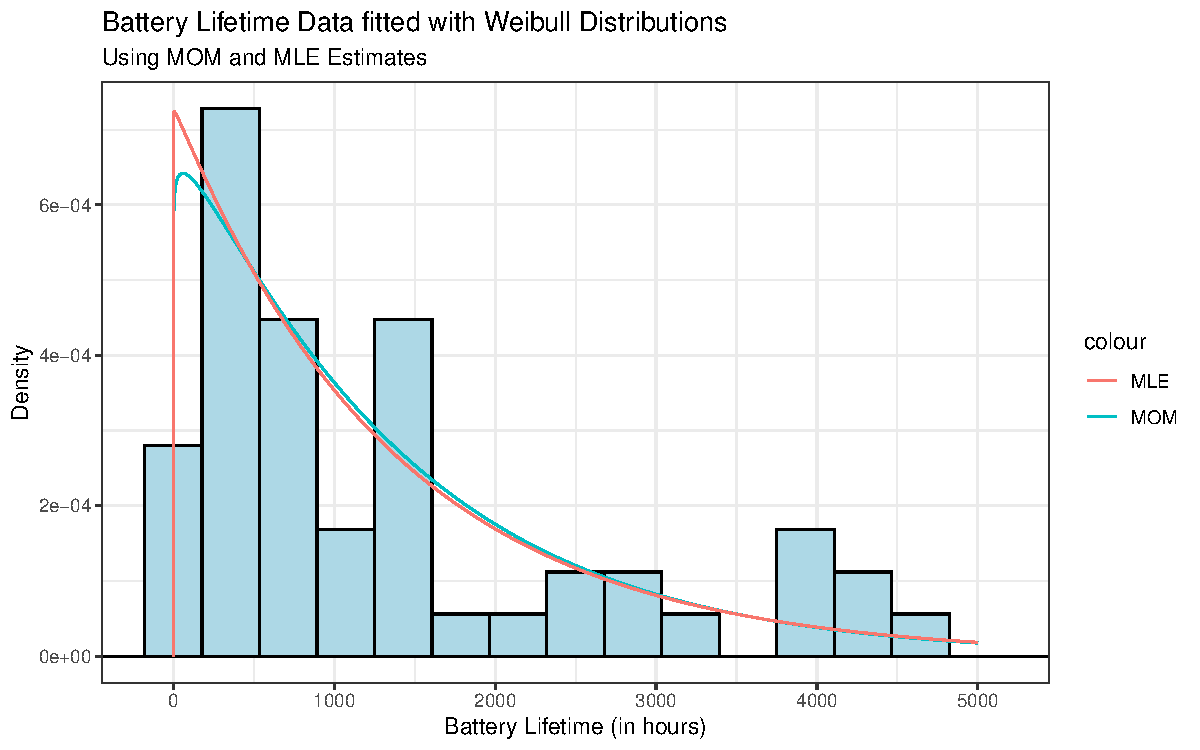
\includegraphics{HW2-005}
\newline
\cite{ggplot}
\cite{gridExtra}
\newline
As you can see from the graph, the red line is the MOM Weibull distribution and the black line is the MLE Weibull distribution. Both lines graph very similar relationships where the lifetime of a battery starts out positive and decreases exponentially. The main difference between these lines can be seen when estimating the initial lifetime of the battery at 0 hours. The MOM estimate shows a more conservative estimate than the MLE estimate, however the MLE estimate is more in line with the actual data we observed. From this, we further illustrate that the MLE method is more accurate for point estimation than the MOM method. 
\newline
\newline
Failed Attempt:
\newline
I misunderstood what the question was asking but found a cool package that could be useful in the future!
\begin{Schunk}
\begin{Sinput}
> #install.packages("fitdistrplus")
> library(fitdistrplus) #fit distribution
> fw<-fitdist(dat.battery, "weibull")
> summary(fw)
> #shape = 1.003388
> #scale = 1358.094597
> weibull.dist<-data.frame(x=c(0:5000), 
+                          f=dweibull(x=(0:5000),
+                           shape=1.003388, 
+                           scale=1358.094597, 
+                           log=FALSE))
\end{Sinput}
\end{Schunk}
  \item \textbf{In Example 7.9 and Example 7.16 in the notes, we found the MOM and MLE
  for this data when modelled by the exponential distribution. Consider the following
  calculation and discuss which model fits better.}
  \[ \frac{L(\lambda|\mathbf{x})}{L(\eta,\beta|\mathbf{x})}.\]
  \textbf{Solution:}
  \newline
MOM:
\newline
\begin{Schunk}
\begin{Sinput}
> prod(dexp(dat.battery, rate= .0007375393))/
+   prod(dweibull(dat.battery, shape = 1.039419, scale = 1377.130555))
\end{Sinput}
\begin{Soutput}
[1] 1.05219
\end{Soutput}
\end{Schunk}
The above calculation divides the likelihood of the exponential distribution by the likelihood of the weibull distribution using MOM estimates. Since the function is greater than 1, we know that the exponential distribution is a better estimate in this case. 

MLE:
\begin{Schunk}
\begin{Sinput}
> 410.6096/410.6091
\end{Sinput}
\begin{Soutput}
[1] 1.000001
\end{Soutput}
\begin{Sinput}
> #1.000001
\end{Sinput}
\end{Schunk}
The above calculation divides the log likelihood of one parameter lambda given x by the log likelihood of two parameters, eta and beta, given x. This means that the above calculation is referencing the likelihood, found from the MLE method, of both distributions. The likelihood value of the weibull distribution is 410.6091. The likelihood value of the exponential distribution is 410.6096. These likelihood values therefore are essentially the same, since the .0005 difference is most likely negligible and the fraction above comes out to be a value very close to 1.
  
\end{enumerate}
\newpage
%%%%%%%%%%%%%%%%%%%%%%%%%%%%%%%%%%%%%%%%%%%%%%%%%%%%%%%%%%%%%%%%%%%%%%%%%%%%%%
%%%%%%%%%%%%%%%%%%%%%%%%%%%%%%%%%%%%%%%%%%%%%%%%%%%%%%%%%%%%%%%%%%%%%%%%%%%%%%%
%%%%%%%%%  Question 3
%%%%%%%%%%%%%%%%%%%%%%%%%%%%%%%%%%%%%%%%%%%%%%%%%%%%%%%%%%%%%%%%%%%%%%%%%%%%%%%
%%%%%%%%%%%%%%%%%%%%%%%%%%%%%%%%%%%%%%%%%%%%%%%%%%%%%%%%%%%%%%%%%%%%%%%%%%%%%%%
\item \textbf{(Central Limit Theorem)} Demonstrate the Central Limit Theorem.
Simulate $X_1, X_2, ..., X_n$ from each distribution $r=1000$ times. Calculate
$\bar{X}$ for each simulation, plot their histogram and overlay a graph of the 
Gaussian density with mean and standard deviation as specified by the Central 
Limit Theorem.
  \begin{enumerate}
    \item Choose what type of loop is necessary for this exercise.
    \newline
    \textbf{Solution:}
    \newline
    A for loop is necessary for this exercise because a for loop is a definite loop. A for loop iterates over a set of values or objects and ends when it reachs the end of the sequence. Since we have a set number of iterations (1000), a for loop would be best for calculating and storing 1000 sample means. 
    \item The Central Limit Theorem states that as $n$ increases
    \[\bar{X}_n = \frac{1}{n} \sum_{i=1}^n {X} \sim \mathcal{AG}\left(\mu_{\bar(x)} = E(X), \sigma_{\bar(x)} = \frac{sd(X)}{\sqrt{n}}\right).\]
    Write out this statement for the sample of $n$ observations drawn from 
    \begin{enumerate}
      \item the Gaussian($\mu_x=0$, $\sigma_x=1$) distribution
      \newline
      \textbf{Solution:}
      \newline
      \[\bar{X}_n = \frac{1}{n} \sum_{i=1}^n {X} \sim \mathcal{AG}\left(\mu_{\bar(x)} = 0, \sigma_{\bar(x)} = \frac{1}{\sqrt{n}}\right).\] 
      \item the Uniform($a=0$, $b=1$) distribution
      \newline
      \textbf{Solution:}
      \newline
       \[\bar{X}_n = \frac{1}{n} \sum_{i=1}^n {X} \sim \mathcal{AG}\left(\mu_{\bar(x)} = \frac{1}{2}, \sigma_{\bar(x)} = \frac{1}{2\sqrt{3n}}\right).\]
      \item the Exponential($\lambda=5$) distribution (Example 7.4 in notes)
      \newline
      \textbf{Solution:}
      \newline
      \[\bar{X}_n = \frac{1}{n} \sum_{i=1}^n {X} \sim \mathcal{AG}\left(\mu_{\bar(x)} = \frac{1}{5}, \sigma_{\bar(x)} = \frac{1}{5\sqrt{n}} \right).\]
      \item the Poisson($\lambda=5$).
      \newline
      \textbf{Solution:}
      \newline
      \[\bar{X}_n = \frac{1}{n} \sum_{i=1}^n {X} \sim \mathcal{AG}\left(\mu_{\bar(x)} = 5, \sigma_{\bar(x)} = \sqrt{\frac{5}{n}}\right).\]
    \end{enumerate} 
    This will be the Gaussian curve you will overlay on the histogram.
\newline
\newline
Failed Attempts:
\newline
Here, I did not understand at first if the problem should be answered using LaTex or R. 
\begin{Schunk}
\begin{Sinput}
> #Gaussian(0,1)
> sample.mean.Gaus<-function(n){
+   (1/n)*(sum(dnorm(x=n,mean = 0, sd=1,log = FALSE)))
+ }
\end{Sinput}
\end{Schunk}
\begin{Schunk}
\begin{Sinput}
> #Uniform(a=0, b=1)
> sample.mean.Unif<-function(n){
+   (1/n)*(sum(dunif(x=n,min = 0,max = 1,log=FALSE)))
+ }
\end{Sinput}
\end{Schunk}
\begin{Schunk}
\begin{Sinput}
> #Exponential(lambda=5)
> sample.mean.Exp<-function(n){
+   (1/n)*(sum(dexp(x=n,rate = 5,log=FALSE)))
+ }
\end{Sinput}
\end{Schunk}
\begin{Schunk}
\begin{Sinput}
> #Poisson(lambda=5)
> sample.mean.Pois<-function(n){
+   (1/n)*(sum(dpois(x=n, lambda = 5, log = FALSE)))
+ }
\end{Sinput}
\end{Schunk}
    \item Code a loop that generates $n$ observations drawn from each distribution
    of interest, calculates the sample mean of those observations and stores it.
    Finally, plot a histogram of the saved sample means with an
    overlay of the Gaussian curve from (b) for $n=1,3,10,20,50,100$.
  \begin{table}[H]
	  \begin{center}
		  \begin{tabular} {|l|c|c|c|c|} \hline
			    n & Exponential  & Uniform   & Gaussian & Poisson\\\hline\hline
			    1 & Right-skewed & Symmetric & Bell-shaped & Symmetric\\
			    3 & Right-skewed & Symmetric & Bell-shaped & Slightly left-skewed\\
			    10& Right-skewed & Symmetric & Bell-shaped & Left-skewed\\
			    20& Right-skewed, Leptokurtic & Symmetric, Leptokurtic & Bell-shaped, Leptokurtic & Slightly left-skewed, Lepto.\\
			    50& Right-skewed, Leptokurtic & Gaussian, Leptokurtic & Bell-shaped, Leptokurtic & Slightly left-skewed, Lepto.\\
			    100& Right-skewed, Leptokurtic & Gaussian, Leptokurtic & Bell-shaped, Leptokurtic & Slightly left-skewed, Lepto.\\\hline
		  \end{tabular}
		  \caption{Shape of the distribution of sample means for the 
		  Exponential($\lambda$=5), Uniform($a=0$, $b=1$), Gaussian($\mu_x=0$, $\sigma-x=1$), and Poisson($\lambda=5$) distributions
		  across $n$.}\label{psim}
	  \end{center}
  \end{table}
  \textbf{Solution:}
  \newline
It's important to note that for my own organization, I used four sets of four loops for the problem so that it would be easier to plot the data. However, this can all be written within one for loop.
\begin{Schunk}
\begin{Sinput}
> #gaussian distribution
> n<-c(1,3,10,20,50,100)
> norm.means1<-c(NA,1000)
> norm.means3<-c(NA,1000)
> norm.means10<-c(NA,1000)
> norm.means20<-c(NA,1000)
> norm.means50<-c(NA,1000)
> norm.means100<-c(NA,1000)
> for (i in n){ #iterate over the wanted sample sizes
+   for (j in 1:1000){ #find sample means 1000 times per n
+     if (i==1){ #sample size 1
+     norm.means1[j]<-mean(rnorm(j,0,1))
+     } else if (i==3) {#sample size 3
+       norm.means3[j]<-mean(rnorm(j,0,1))
+     } else if (i==10) {#sample size 10
+       norm.means10[j]<-mean(rnorm(j,0,1))
+     } else if (i==20) {#sample size 20
+       norm.means20[j]<-mean(rnorm(j,0,1))
+     } else if (i==50) {#sample size 50
+       norm.means50[j]<-mean(rnorm(j,0,1))
+     } else if (i==100) {#sample size 100
+       norm.means100[j]<-mean(rnorm(j,0,1))
+     }
+     
+ }}
\end{Sinput}
\end{Schunk}
\textbf{Normally Distributed Means}
\newline
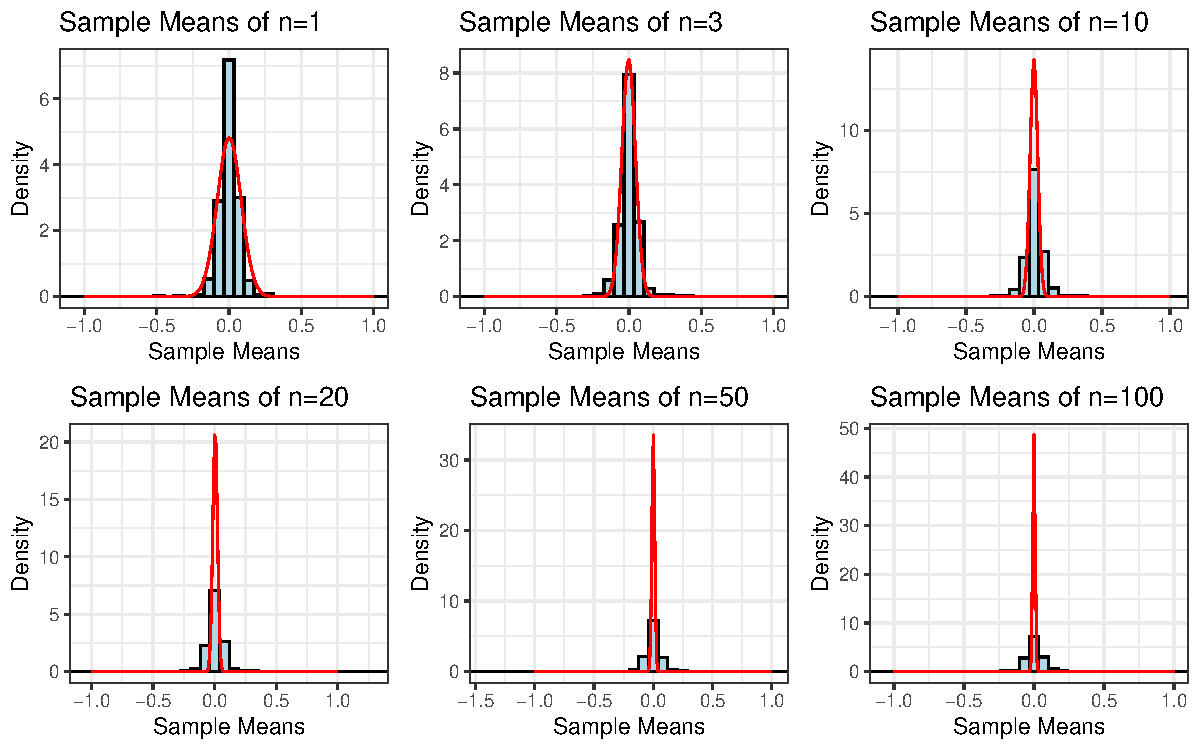
\includegraphics{HW2-014}

\begin{Schunk}
\begin{Sinput}
> #uniform distribution
> n<-c(1,3,10,20,50,100)
> unif.means1<-c(NA,1000)
> unif.means3<-c(NA,1000)
> unif.means10<-c(NA,1000)
> unif.means20<-c(NA,1000)
> unif.means50<-c(NA,1000)
> unif.means100<-c(NA,1000)
> for (i in n){ #specify desired sample size
+   for (j in 1:1000){ #1000 iterations
+     if (i==1){
+     unif.means1[j]<-mean(runif(j,0,1))
+     } else if (i==3) {
+       unif.means3[j]<-mean(runif(j,0,1))
+     } else if (i==10) {
+       unif.means10[j]<-mean(runif(j,0,1))
+     } else if (i==20) {
+       unif.means20[j]<-mean(runif(j,0,1))
+     } else if (i==50) {
+       unif.means50[j]<-mean(runif(j,0,1))
+     } else if (i==100) {
+       unif.means100[j]<-mean(runif(j,0,1))
+     }
+     
+ }}
\end{Sinput}
\end{Schunk}
\newpage
\textbf{Uniformly Distributed Means}
\newline
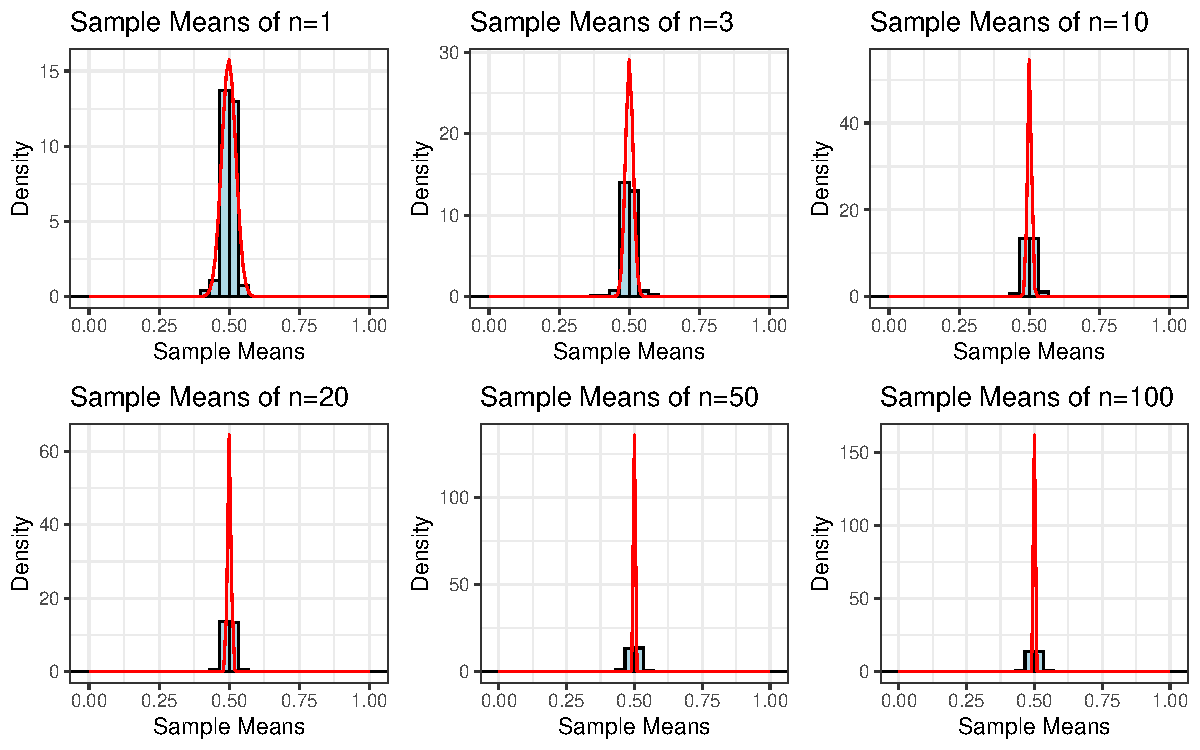
\includegraphics{HW2-016}

\begin{Schunk}
\begin{Sinput}
> #exponential distribution
> n<-c(1,3,10,20,50,100)
> exp.means1<-c(NA,1000)
> exp.means3<-c(NA,1000)
> exp.means10<-c(NA,1000)
> exp.means20<-c(NA,1000)
> exp.means50<-c(NA,1000)
> exp.means100<-c(NA,1000)
> for (i in n){
+   for (j in 1:1000){
+     if (i==1){
+     exp.means1[j]<-mean(rexp(j,5))
+     } else if (i==3) {
+       exp.means3[j]<-mean(rexp(j,5))
+     } else if (i==10) {
+       exp.means10[j]<-mean(rexp(j,5))
+     } else if (i==20) {
+       exp.means20[j]<-mean(rexp(j,5))
+     } else if (i==50) {
+       exp.means50[j]<-mean(rexp(j,5))
+     } else if (i==100) {
+       exp.means100[j]<-mean(rexp(j,5))
+     }
+     
+ }}
\end{Sinput}
\end{Schunk}
\newpage
\textbf{Exponentially Distributed Means}
\newline
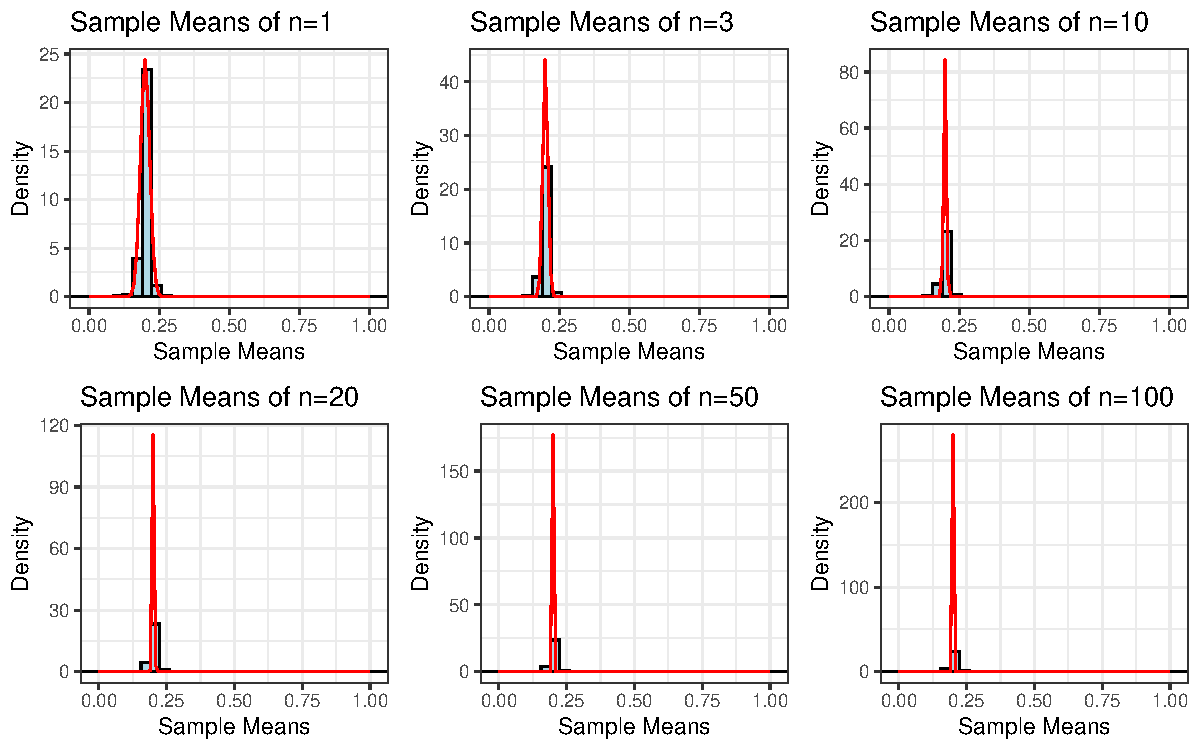
\includegraphics{HW2-018}

\begin{Schunk}
\begin{Sinput}
> #poisson distribution
> n<-c(1,3,10,20,50,100)
> pois.means1<-c(NA,1000)
> pois.means3<-c(NA,1000)
> pois.means10<-c(NA,1000)
> pois.means20<-c(NA,1000)
> pois.means50<-c(NA,1000)
> pois.means100<-c(NA,1000)
> for (i in n){
+   for (j in 1:1000){
+     if (i==1){
+     pois.means1[j]<-mean(rpois(j,5))
+     } else if (i==3) {
+       pois.means3[j]<-mean(rpois(j,5))
+     } else if (i==10) {
+       pois.means10[j]<-mean(rpois(j,5))
+     } else if (i==20) {
+       pois.means20[j]<-mean(rpois(j,5))
+     } else if (i==50) {
+       pois.means50[j]<-mean(rpois(j,5))
+     } else if (i==100) {
+       pois.means100[j]<-mean(rpois(j,5))
+     }
+     
+ }}
\end{Sinput}
\end{Schunk}
\newpage
\textbf{Poisson Distributed Means}
\newline
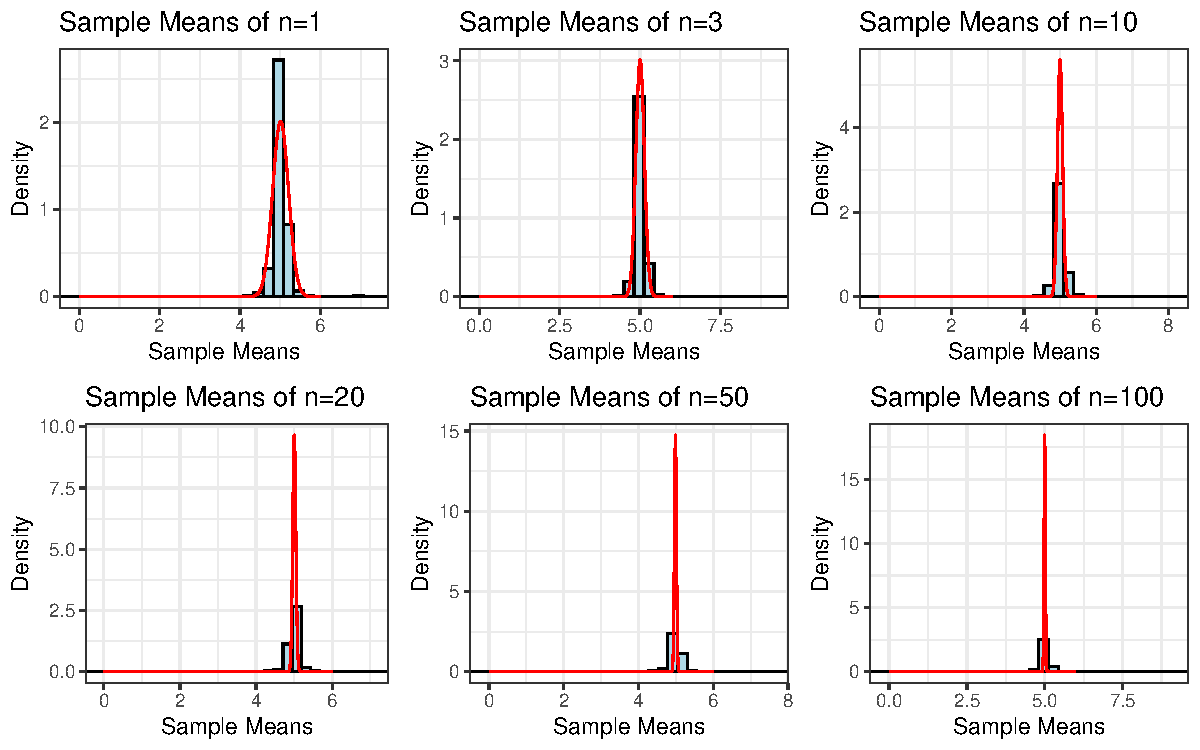
\includegraphics{HW2-020}

Failed Attempt:
\begin{Schunk}
\begin{Sinput}
> # functions = c(rnorm, runif, rexp, rpois)
> # for (i in functions){
> #   for (i in 1:1000){
> #     functions.means[i]<-mean(functions(1000,0,1))
> #   }
> # }
\end{Sinput}
\end{Schunk}
This approach did not work because rnorm, runif, rexp, and rpois both have different numbers of input and different inputs in general. While I could've had 2 for loops instead of four, and group together rnorm and runif, and rexp and rpois, for the sake of organization and readable of code I decided to give each function its own for loop.

\begin{Schunk}
\begin{Sinput}
> #uniform distribution
> unif.means<-rep(NA,1000)
> for (i in 1:1000){
+   unif.means[i]<-mean(runif(i,0,1))
+ }
\end{Sinput}
\end{Schunk}

\begin{Schunk}
\begin{Sinput}
> #exponential distribution
> exp.means<-rep(NA,1000)
> for (i in 1:1000){
+   exp.means[i]<-mean(rexp(i, rate = 5))
+ }
\end{Sinput}
\end{Schunk}

\begin{Schunk}
\begin{Sinput}
> #poisson distribution
> pois.means<-rep(NA,1000)
> for (i in 1:1000){
+   pois.means[i]<-mean(rpois(i,lambda = 5))
+ }
\end{Sinput}
\end{Schunk}
  \item Discuss the results of this simulation with respect to the Central Limit Theorem.
  \newline
  \newline
  \textbf{Solution:}
  \newline
  This simulation is supposed mimic the Central Limit Theorem, meaning that as n increases, the distribution of the parameter is supposed to become more Gaussian. For this simulation, we increased n to 1,3,10,20,50,100 for the Gaussian, Uniform, Exponential, and Poisson Distributions. We can see that the Gaussian distribution stayed Gaussian and became more leptokurtic as n increased. For the Uniform distribution, it was symmetric and approximately gaussian, and more leptokurtic as n increased. The Exponential distribution remained right-skewed, but become more Gaussian and leptokurtic as n increased. The Poisson distribution was left skewed, but became more Gaussian and leptokurtic as n increased. All distributions became more leptokurtic because as n increased, standard error decreased. 
  \end{enumerate}
\newpage
%%%%%%%%%%%%%%%%%%%%%%%%%%%%%%%%%%%%%%%%%%%%%%%%%%%%%%%%%%%%%%%%%%%%%%%%%%%%%%%
%%%%%%%%%%%%%%%%%%%%%%%%%%%%%%%%%%%%%%%%%%%%%%%%%%%%%%%%%%%%%%%%%%%%%%%%%%%%%%%
%%%%%%%%%  Question 4
%%%%%%%%%%%%%%%%%%%%%%%%%%%%%%%%%%%%%%%%%%%%%%%%%%%%%%%%%%%%%%%%%%%%%%%%%%%%%%%
%%%%%%%%%%%%%%%%%%%%%%%%%%%%%%%%%%%%%%%%%%%%%%%%%%%%%%%%%%%%%%%%%%%%%%%%%%%%%%%
\item \textbf{(Central Limit Theorem)} The time to death for rats injected with a toxic substance, denoted by $Y$
	(measured in days), follows an exponential distribution with $\lambda = 1/5$. That is,
	\[Y \sim \textrm{exponential}(\lambda = 1/5).\]
	This is the population distribution. It describes the time to death for all individual rats
	in the population.
	\begin{enumerate}
	  \item Plot the exponential$(\lambda = 1/5)$ population distribution.
	  \newline
	  \textbf{Solution:}
\begin{Schunk}
\begin{Sinput}
> x<-seq(0,25,0.01)
> ggdat<-data.frame(x=x,
+                   f.pop=dexp(x,1/5))
> ggplot(data=ggdat, aes(x=x, y=f.pop))+
+   geom_line(color="black")+
+   theme_bw()+
+   geom_hline(yintercept = 0)+
+   xlab("x")+
+   ylab("Density")+
+   ggtitle("Population Distribution for Exponential Distribution")
\end{Sinput}
\end{Schunk}
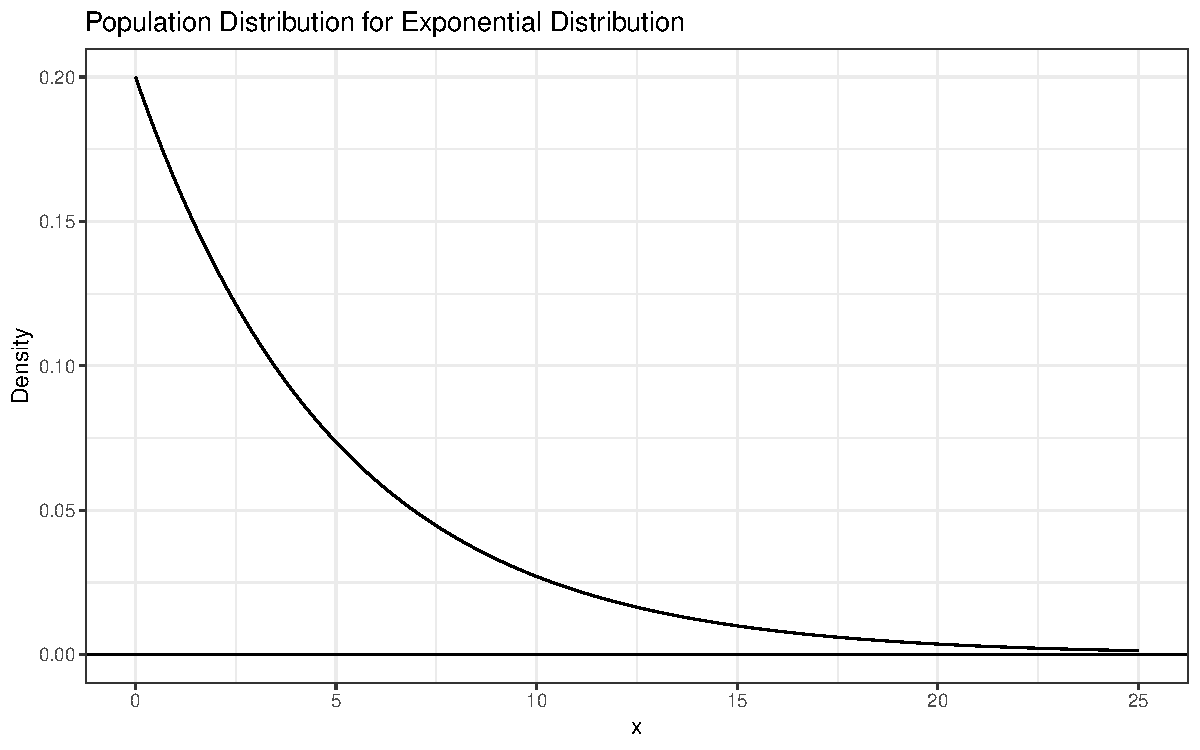
\includegraphics{HW2-025}
	  \item The theoretical sampling distributions of $\bar{Y}$ is gamma($\alpha=n$,$\beta=\frac{1}{n\lambda}$). 
	  You can ask \texttt{R} for the gamma distribution using \texttt{dgamma(x=x,shape=n,scale=1/(n*lambda))}.
	  Plot the theoretical distribution for $n=2$, $n=10$, and $n=35$.
	  \newline
	  \textbf{Solution:}
\begin{Schunk}
\begin{Sinput}
> x<-seq(0,25,0.01)
> n.2<-data.frame(x=x, f.pop=dgamma(x=x,shape=2,scale=1/(2*(1/5))))
> n.10<-data.frame(x=x, f.pop=dgamma(x=x,shape=10,scale=1/(10*(1/5))))
> n.35<-data.frame(x=x, f.pop=dgamma(x=x,shape=35,scale=1/(35*(1/5))))
> ggplot(data=ggdat, aes(x=x, y=f.pop))+
+   geom_line(data=n.2, aes(x=x, y=f.pop, color="n=2"))+
+   geom_line(data=n.10, aes(x=x, y=f.pop, color="n=10"))+
+   geom_line(data=n.35, aes(x=x, y=f.pop, color="n=35"))+
+   theme_bw()+
+   xlab("x")+
+   ylab("Density")+
+   ggtitle("Population Distributions for Gamma Distribution", 
+           subtitle = "for n=2, n=10, n=35")
\end{Sinput}
\end{Schunk}
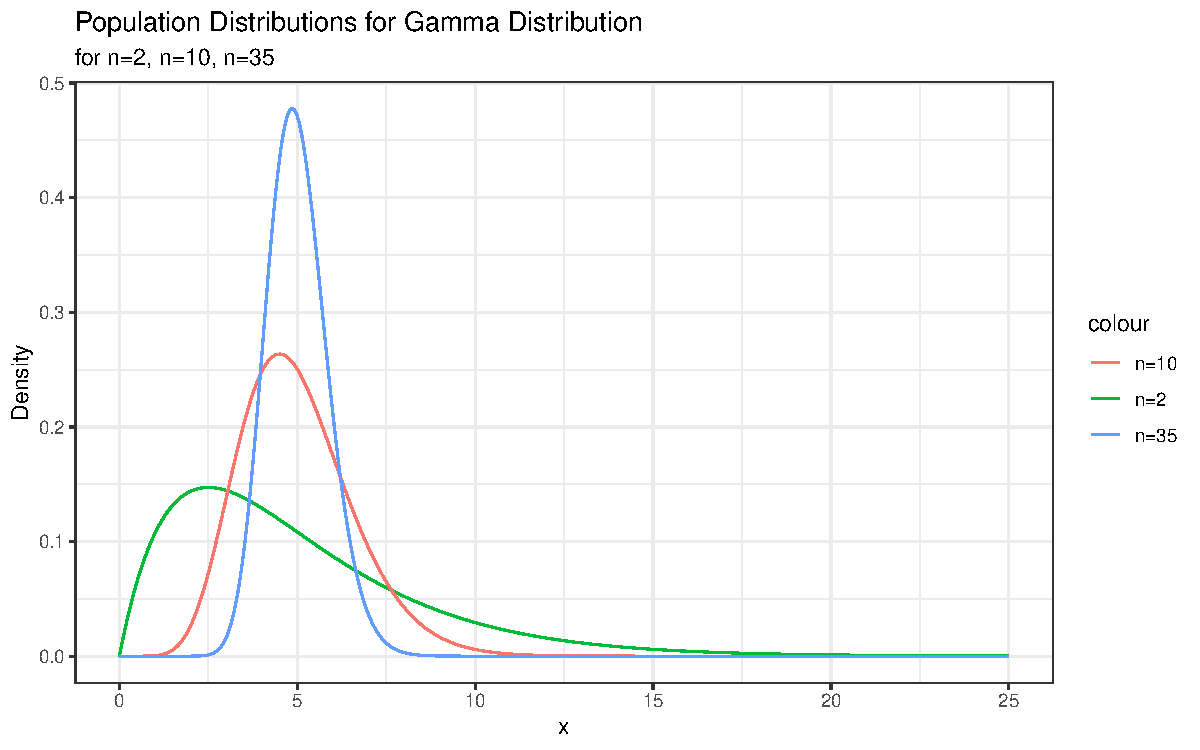
\includegraphics{HW2-026}
\newline
For reference, we can see that as the sampe size increases, the gamma distribution becomes more normally distributed.
	  \item The Central Limit Theorem says that as $n$ increases, the sampling distribution of $\bar{X}$ can
	  be well approximated with a Gaussian distribution. Superimpose the approximate sampling distribution of $\bar{X}$
	  for $n=2$, $n=10$, and $n=35$.
\newline
\textbf{Solution:}
\newline
\begin{Schunk}
\begin{Sinput}
> x<-seq(0,12,0.01)
> gamma2<-data.frame(x=x, f.pop=dgamma(x=x,shape=2,scale=1/(2*(1/5))))
> gamma10<-data.frame(x=x, f.pop=dgamma(x=x,shape=10,scale=1/(10*(1/5))))
> gamma35<-data.frame(x=x, f.pop=dgamma(x=x,shape=35,scale=1/(35*(1/5))))
> norm2<-data.frame(x=x, y=dnorm(x, mean = 5, sd= (1/(1/5))/sqrt(2)))
> norm10<-data.frame(x=x, y=dnorm(x, mean = 5, sd= (1/(1/5))/sqrt(10)))
> norm35<-data.frame(x=x, y=dnorm(x, mean = 5, sd= (1/(1/5))/sqrt(35)))
> ggplot(data=ggdat, aes(x=x, y=f.pop))+
+   geom_line(data=gamma2, aes(x=x, y=f.pop, color="Gamma n=2"))+
+   geom_line(data=gamma10, aes(x=x, y=f.pop, color="Gamma n=10"))+
+   geom_line(data=gamma35, aes(x=x, y=f.pop, color="Gamma n=35"))+
+   geom_line(data=norm2, aes(x=x, y=y, color="Normal n=2"))+
+   geom_line(data=norm10, aes(x=x, y=y, color="Normal n=10"))+
+   geom_line(data=norm35, aes(x=x, y=y, color="Normal n=35"))+
+   theme_bw()+
+   xlab("x")+
+   ylab("Density")+
+   ggtitle("Population Distributions for Gamma and Normal Distributions", 
+           subtitle = "for n=2, n=10, n=35")
>   #scale_color_discrete(name="Distribution/Sample Size", labels=c("ggdat2","ggdat10","ggdat35", "ggdat2n", "ggdat10n", "ggdat35n"))
\end{Sinput}
\end{Schunk}
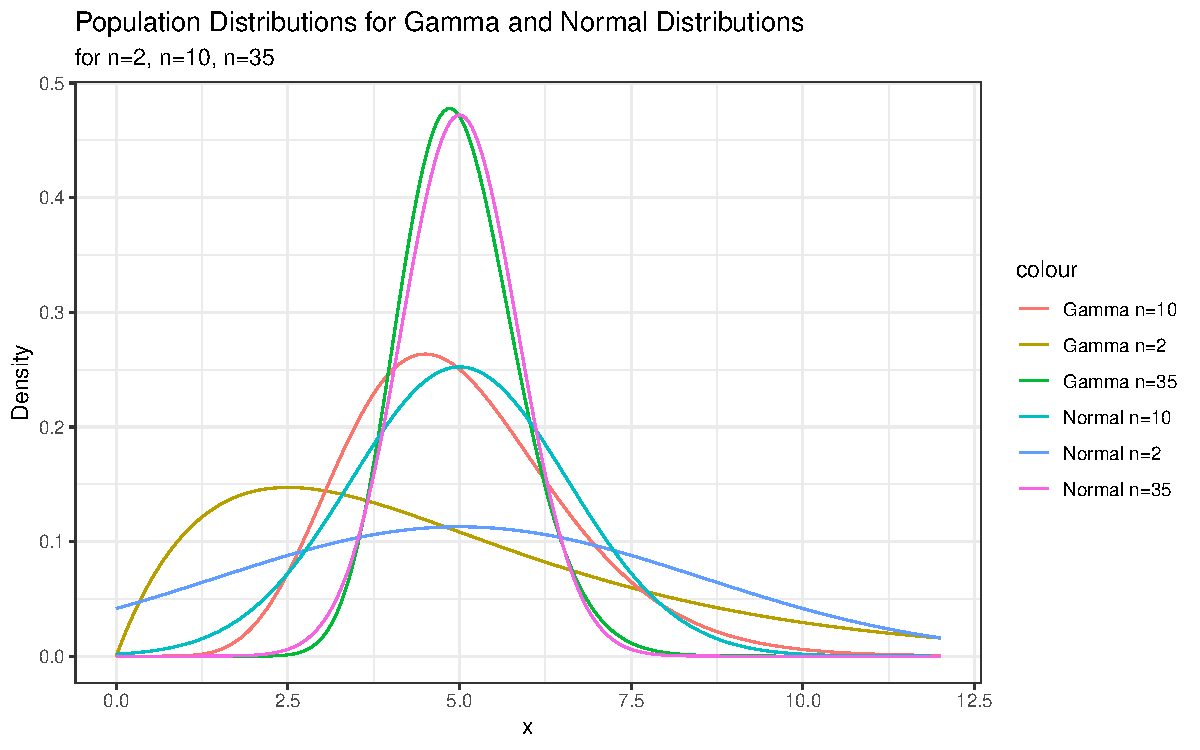
\includegraphics{HW2-027}
%sd = 1/lambda
%se = sd/sqrt(n)
%se = (1/lambda)/sqrt(n)
\newline
As you can see, the gamma distribution becomes approximately gaussian as the sample size increases. As you can see, the lines representing n=2 have distrinctly different curves. However, when n=10, the lines are similar. At n=35, the lines representing the gamma distribution almost overlap. This illustrates that as the sample size increases, the gamma distribution means become approximately gaussian distributed. 
	  \item Find the probability that a randomly selected rat injected with the toxic substance
	  lives longer than 1 day.
	  \newline
	  \textbf{Solution:}
\begin{Schunk}
\begin{Sinput}
> #P(X > 1)
> rat.life.1.day<-1-pexp(1,1/5)
> pexp(1,1/5,lower.tail = FALSE)
\end{Sinput}
\begin{Soutput}
[1] 0.8187308
\end{Soutput}
\end{Schunk}
The probability that a randomly selected rat injected with the toxic substance lives longer than a day is 81.87\%.
	  \item Find the probability that a randomly selected rat injected with the toxic substance
	  lives between 1 and 3 days.
	  \newline
	  \textbf{Solution:}
\begin{Schunk}
\begin{Sinput}
> #P(X > 1 & X < 3)
> #P(X > 1)
> rat.life.1.day<-pexp(1,1/5,lower.tail=FALSE)
> #P(X > 3)
> rat.life.3.day<-pexp(3,1/5,lower.tail = FALSE)
> rat.life.1.day-rat.life.3.day
\end{Sinput}
\begin{Soutput}
[1] 0.2699191
\end{Soutput}
\end{Schunk}
The probability that a randomly selected rat injected with the toxic substance lives between 1 and 3 days is 26.99\%. 
	  \item Find the probability that a randomly selected rat injected with the toxic substance
	  lives longer than 1 week.
	  \newline
	  \textbf{Solution:}
\begin{Schunk}
\begin{Sinput}
> #P(X > 7)
> pexp(7,1/5,lower.tail=FALSE)
\end{Sinput}
\begin{Soutput}
[1] 0.246597
\end{Soutput}
\end{Schunk}
The probability that a randomly selected rat lives longer than 1 week is 24.66\%.
	  \item Find the exact probability, using the gamma distribution, that two randomly selected 
	  rats injected with the toxic substance live longer than 1 day on average.
	  \newline
	  \textbf{Solution:}
\begin{Schunk}
\begin{Sinput}
> #two randomly selected rats, 1 day
> #P(X > 1|n=2)
> pgamma(1,shape=2,scale=1/(2*(1/5)),lower.tail = FALSE)
\end{Sinput}
\begin{Soutput}
[1] 0.9384481
\end{Soutput}
\end{Schunk}
%ag norm takes sd and mean from exp
%sd of ag norm sd/rad n
The exact probability that two randomly selected rats injected with the toxic substance live longer than 1 day on average is 93.84\%.
	  \item Find the approximate probability, using the Central Limit Theorem, that two randomly 
	  selected rats injected with the toxic substance live longer than 1 day on average.
	  \newline
	  \textbf{Solution:}
\begin{Schunk}
\begin{Sinput}
> #two rats randomly selected -> independence
> pnorm(1,mean = 1/(1/5),sd= (1/(1/5))/sqrt(2),lower.tail = FALSE)
\end{Sinput}
\begin{Soutput}
[1] 0.8710505
\end{Soutput}
\end{Schunk}
The approximate probability, using the Central Limit Theorem, that two randomly selected rats injected with the toxic substance live longer than 1 day on average is 87.11\%.
	  \item Find the exact probability, using the gamma distribution, that two randomly selected 
	  rats injected with the toxic substance live  between 1 and 3 days on average.
	  \newline
	  \textbf{Solution:}
\begin{Schunk}
\begin{Sinput}
> #P(X>1 and X<3)
> #P(X>1)
> rat.life.1.day<-pgamma(1,shape = 2,scale = 1/(2*(1/5)),lower.tail = FALSE)
> #P(X>3)
> rat.life.3.day<-pgamma(3,shape=2,scale=(1/(2*(1/5))),lower.tail = FALSE)
> rat.life.1.day-rat.life.3.day
\end{Sinput}
\begin{Soutput}
[1] 0.2758208
\end{Soutput}
\end{Schunk}
The exact probability using the gamma distribution that two randomly selected rats injected with the toxic substance live between 1 and 3 days on average is 27.58\%.
	  \item Find the approximate probability, using the Central Limit Theorem, that two randomly 
	  selected rats injected with the toxic substance live between 1 and 3 days on average.
	  \newline
	  \textbf{Solution:}
\begin{Schunk}
\begin{Sinput}
> #two rats randomly selected -> independence
> #P(X>1)
> rat.life.1.day<-1-pnorm(1,mean = 1/(1/5),sd= (1/(1/5))/sqrt(2))
> #P(X<3)
> rat.life.3.day<-1-pnorm(3,mean = 1/(1/5),sd= (1/(1/5))/sqrt(2))
> rat.life.1.day-rat.life.3.day
\end{Sinput}
\begin{Soutput}
[1] 0.1568543
\end{Soutput}
\end{Schunk}
The approximate probability, using the Central Limit Theorem, that two randomly selected rats injected with the toxic substance live between 1 and 3 days on average, is 15.69\%.
  \end{enumerate}

\newpage
%%%%%%%%%%%%%%%%%%%%%%%%%%%%%%%%%%%%%%%%%%%%%%%%%%%%%%%%%%%%%%%%%%%%%%%%%%%%%%%
%%%%%%%%%%%%%%%%%%%%%%%%%%%%%%%%%%%%%%%%%%%%%%%%%%%%%%%%%%%%%%%%%%%%%%%%%%%%%%%
%%%%%%%%%  Question 5
%%%%%%%%%%%%%%%%%%%%%%%%%%%%%%%%%%%%%%%%%%%%%%%%%%%%%%%%%%%%%%%%%%%%%%%%%%%%%%%
%%%%%%%%%%%%%%%%%%%%%%%%%%%%%%%%%%%%%%%%%%%%%%%%%%%%%%%%%%%%%%%%%%%%%%%%%%%%%%%
\item \textbf{(Inference)} Assume that an alien has landed on Earth and wants to understand the gender diversity of humans.
Fortunately, the alien took a good statistics course on its home planet, so it knows to take a sample 
of human beings and produce a confidence interval for this proportion.  Unfortunately, the alien happens 
upon the 2019 US Senate as its sample of human beings.  The US Senate has 25 senators who self-identify as 
having a female gender (its most ever!) among its 100 members in 2019.
\begin{enumerate}
\item Calculate the alien's 95\% confidence interval.
\newline
\textbf{Solution:}
\begin{Schunk}
\begin{Sinput}
> #install.packages("binom")
> library(binom)
> binom.confint(25,100,conf.level = 0.95)
\end{Sinput}
\begin{Soutput}
          method  x   n      mean     lower     upper
1  agresti-coull 25 100 0.2500000 0.1749621 0.3435347
2     asymptotic 25 100 0.2500000 0.1651311 0.3348689
3          bayes 25 100 0.2524752 0.1700590 0.3376355
4        cloglog 25 100 0.2500000 0.1701718 0.3378379
5          exact 25 100 0.2500000 0.1687797 0.3465525
6          logit 25 100 0.2500000 0.1749063 0.3438965
7         probit 25 100 0.2500000 0.1732088 0.3418503
8        profile 25 100 0.2500000 0.1721511 0.3405078
9            lrt 25 100 0.2500000 0.1721635 0.3405060
10     prop.test 25 100 0.2500000 0.1711755 0.3483841
11        wilson 25 100 0.2500000 0.1754521 0.3430446
\end{Soutput}
\end{Schunk}
\cite{binom}
\newline
Using the Wilson method, the alien's confidence interval with 95\% confidence is (0.1754521, 0.3430446).
\item Interpret the interval.
\newline
\textbf{Solution:}
\newline
The alien is confident that the true population mean of self-identifying female human beings on Earth is between 17.55\% and 34.30\%, 95\% of the time. 
\newline
\item Is this consistent with your experience living on this planet?
\newline
\textbf{Solution:}
\newline
This is not consistent with my experience living on this planet. I pretty much assume that around half of the people on the planet are women and half of the people on the planet are men. 
\newline
\item What went wrong?
\newline
\textbf{Solution:}
\newline
The real issue is that this was not a representative sample, and therefore the interval cannot be generalized to human population. The US Senate (believe it or not), is not a good representation of the population of the US even though that is their job and what they're paid for. US senators are also not representative of the world population in regards to gender, and certainly not in other aspects either. A better way to interpret this confidence interval is that the alien is confident that the true population mean of self-identifying female human beings in the US Senate in 2019 is between 17.55\% and 34.30\%, 95\% of the time.
\item As we saw in class, about 5\% of all 95\% confidence intervals fail 
to capture the actual value of the population parameter. Is that the explanation for what went wrong here? 
\newline
\textbf{Solution:}
\newline
That is not the explanation for what went wrong here because the sample itself was already systematically, statistically flawed. We saw in class that about 5\% of all 95\% confidence intervals fail to capture the actual value of the population parameter. However, this applies to confidence intervals taken from random samples, which are inherently representative. As stated before though, this sample is not representative of Earth. This sample is at most representative of the US Senate in 2019. Therefore, if this confidence interval was being used to learn about the US Senate in 2019, it would not be in the 5\% of all 95\% confidence intervals that fail to capture the population parameter. 
\item Would it be reasonable for the alien to conclude, with 95\% confidence, that between 
the percentage of U.S. senators in the year 2019 that self-identify as female is in the
95\% confidence interval from part (a)?
\newline
\textbf{Solution:}
\newline
It would be reasonable for the alien to conclude that their confidence interval contains the true population proportion of U.S. senators in the year 2019 that self-identify as female. It would not be reasonable for the alien to be 95\% confident because that is not what the confidence interval projects. It does not project confidence. It projects the true proportion of the sample. 
\end{enumerate}

\newpage
%%%%%%%%%%%%%%%%%%%%%%%%%%%%%%%%%%%%%%%%%%%%%%%%%%%%%%%%%%%%%%%%%%%%%%%%%%%%%%%
%%%%%%%%%%%%%%%%%%%%%%%%%%%%%%%%%%%%%%%%%%%%%%%%%%%%%%%%%%%%%%%%%%%%%%%%%%%%%%%
%%%%%%%%%  Question 6
%%%%%%%%%%%%%%%%%%%%%%%%%%%%%%%%%%%%%%%%%%%%%%%%%%%%%%%%%%%%%%%%%%%%%%%%%%%%%%%
%%%%%%%%%%%%%%%%%%%%%%%%%%%%%%%%%%%%%%%%%%%%%%%%%%%%%%%%%%%%%%%%%%%%%%%%%%%%%%%
\item \textbf{(Inference)} Below you will load and summarize a dataset 
  containing 575 observations of drug treatments. The data includes the following
  \begin{itemize}
    \item ID --	Identification Code	(1 - 575)
    \item AGE	-- Age at Enrollment	(Years)
    \item BECK -- Beck Depression Score	(0.000 - 54.000)
    \item HC --	Heroin/Cocaine Use During	3 Months Prior to Admission (1 = Heroin
    \& Cocaine; 2 = Heroin Only, 3 = Cocaine Only; 4 = Neither Heroin nor Cocaine)
    \item IV -- History of IV Drug Use	(1 = Never; 2 = Previous; 3 = Recent)
    \item IV3	-- Recent IV use	(1 = Yes; 0 = No)
    \item NDT -- Number of Prior Drug Treatments (0 - 40)
    \item RACE -- Subject's Race	(0 = White; 1 = Non-White)
    \item TREAT -- Treatment Randomization (0 = Short Assignment;	1 = Long Assignment)
    \item SITE -- Treatment Site (0 = A; 1 = B)
    \item LEN.T	-- Length of Stay in Treatment (Days Admission Date to Exit Date)	
    \item TIME -- Time to Drug Relapse (Days Measured from Admission Date)
    \item CENSOR -- Event for Treating Lost to Follow-Up as Returned to Drugs 
    (1 = Returned to Drugs or Lost to Follow-Up; 0 = Otherwise)
    \item etc.
  \end{itemize}
  \begin{enumerate} %this begins a lettered enumerate so I can ask more 
                    %than one question in a question.
    \item Load the data provided in the ``quantreg" package for \texttt{R} \citep{quantreg}.
\begin{Schunk}
\begin{Sinput}
> #install.packages("quantreg",repos = "http://cloud.r-project.org/")
> library("quantreg")
> data("uis")
\end{Sinput}
\end{Schunk}
    \item Is there evidence that patients receiving drug treatments are at least mildly depressed
    on average? That is, is there evidence that the average BECK depression score is greater
    than 13, $\mu>13$?
    \begin{enumerate}
      \item What is the null hypothesis for this test?
      \newline
      \textbf{Solution:}
      \newline
  The null hypothesis is Ho: u = 13. In words, the null hypothesis is that the average Beck Depression Score, the population mean, is equal to 13. 
  \newline
      \item What is the alternative hypothesis for this test?
      \newline
      \textbf{Solution:}
      \newline
  The alternative hypothesis is Ha: u > 13. In words, the alternative hypothesis is that the average Beck Depression Score, the population mean, is greater than 13.
      \newline
      \item What is the sample mean BECK score for these data?
      \newline
      \textbf{Solution:}
\begin{Schunk}
\begin{Sinput}
> mean(uis$BECK)
\end{Sinput}
\begin{Soutput}
[1] 17.36743
\end{Soutput}
\begin{Sinput}
> median(uis$BECK)
\end{Sinput}
\begin{Soutput}
[1] 17
\end{Soutput}
\end{Schunk}
The sample mean BECK score for these data is 17.36743. The sample median BECK score for these data is 17, meaning the data is not too skewed. 
\newline
      \item What is the test statistics for this test?
      \newline
      \textbf{Solution:}
\begin{Schunk}
\begin{Sinput}
> #tstat
> t.stat<-(mean(uis$BECK)-13)/(sd(uis$BECK)/sqrt(length(uis$BECK)))
> #check
> t.test(x=uis$BECK, conf.level = 0.95, mu = 13)
\end{Sinput}
\begin{Soutput}
	One Sample t-test

data:  uis$BECK
t = 11.221, df = 574, p-value < 2.2e-16
alternative hypothesis: true mean is not equal to 13
95 percent confidence interval:
 16.60298 18.13188
sample estimates:
mean of x 
 17.36743 
\end{Soutput}
\end{Schunk}
The test statistic for this test is 11.221.
      \item At what value of $\bar{X}$ does the rejection region start for $\alpha=0.05$?
      \newline
      \textbf{Solution:}
      \newline
\begin{Schunk}
\begin{Sinput}
> qt(.95,574) #1.647513
\end{Sinput}
\begin{Soutput}
[1] 1.647513
\end{Soutput}
\begin{Sinput}
> #solve for xbar
> (1.647513*((sd(uis$BECK))/sqrt(length(uis$BECK))))+13
\end{Sinput}
\begin{Soutput}
[1] 13.64123
\end{Soutput}
\end{Schunk}
The rejection region for $\alpha=0.05$ starts at the value of 13.64123 for $\bar{X}$.
\newline
      \item What is the p value for this test?
      \newline
      \textbf{Solution:}
      \newline
The p value for this test is 2.2e-16 which is essentially zero. Since the p value is less than 0.05, we reject the null hypothesis. 
      \item Graph the results of this test.
\begin{Schunk}
\begin{Sinput}
> ggdat<-data.frame(BECK=uis$BECK)
> ggplot(data = ggdat, aes(x=BECK))+
+   geom_histogram(aes(y=..density..), color='black', fill='lightblue')+
+   xlab("BECK Depression Score")+
+   ylab("Density")+
+   ggtitle("Mean of BECK Depression Score")
\end{Sinput}
\end{Schunk}

\begin{Schunk}
\begin{Sinput}
> x.bar<-mean(uis$BECK)
> mu<-13
> n<-length(uis$BECK)
> alpha<-0.05
> se.xbar<-sd(uis$BECK)/sqrt(n)
> t.obs<-(x.bar-mu)/se.xbar #test statistic
> p.value<-pnorm(abs(t.obs)) #p value
\end{Sinput}
\end{Schunk}

\begin{Schunk}
\begin{Sinput}
> ggdat<-data.frame(t=seq(-15,15,0.01),
+                   f=dt(x=seq(-15,15,0.01),df=574))
> ggdat.obs<-data.frame(x=t.stat, y=0)
> ggdat.highlight<-data.frame(x=qt(p=c(1-alpha/2), df=574),y=c(0,0))
> axis.labels<-round(c(-abs(t.obs),qt(alpha/2,df=n-1),0,qt(1-alpha/2,df=n-1),abs(t.obs))*se.xbar+x.bar,2)
> ggplot(data=ggdat,aes(x=t,y=f))+
+   geom_line()+
+   geom_point(data=ggdat.highlight,aes(x=x,y=y),color="grey")+
+   geom_point(data=ggdat.obs, aes(x=x, y=y), color="red")+
+   geom_ribbon(data=subset(ggdat,t>=qt(1-alpha/2,df=574)), aes(ymax=f), ymin=0,fill="grey",colour=NA, alpha=0.5)+
+     theme_bw()+
+   xlab('t')+
+   ylab("Density")+
+   ggtitle("T Test for BECK Population Mean")+
+   scale_x_continuous(sec.axis = sec_axis(~.,
+                                          breaks=c(-abs(t.obs),qt(alpha/2, n-1),0, qt(1-alpha/2, n-1),abs(t.obs)),
+                                          labels = axis.labels, name="BECK Depression Scores"))
\end{Sinput}
\end{Schunk}
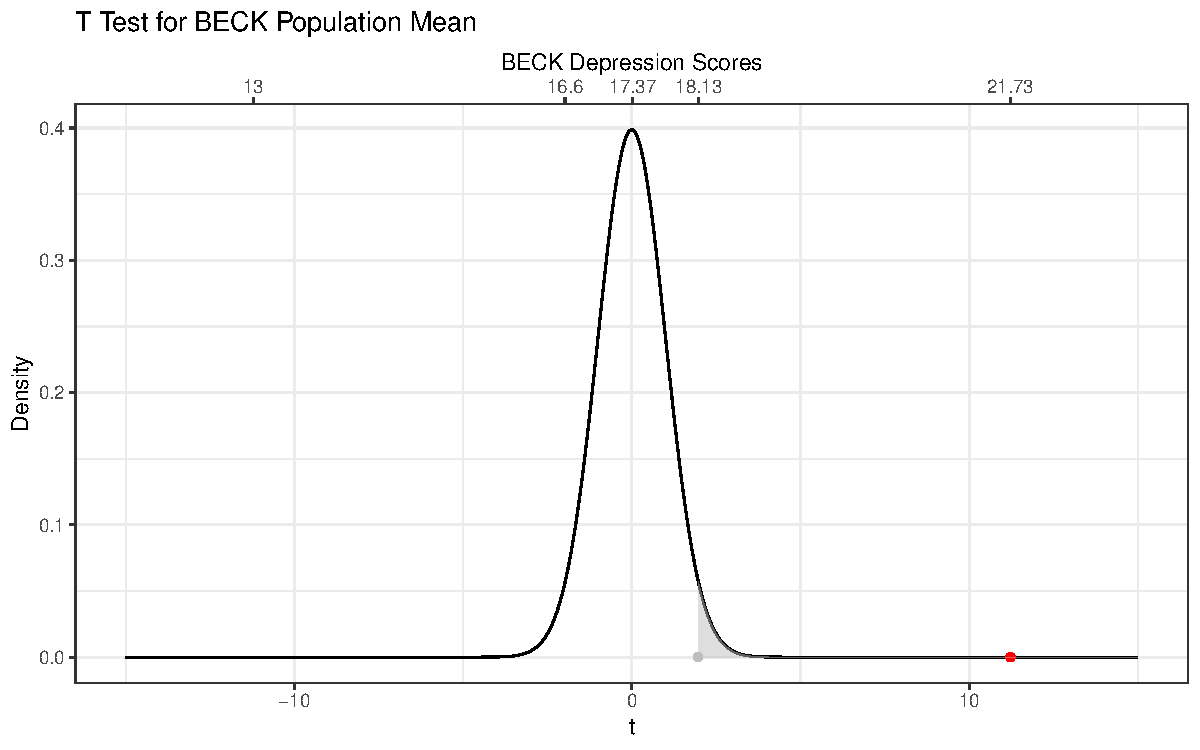
\includegraphics{HW2-042}
\newline
The large degree of freedom, n-1 or 574, emphasizes the leptokurtic shape of the graph. As we can see the red dot is the t value we have, which is statistically significant.
      \item Report a 95\% confidence interval for the average BECK depression score
      and interpret it in the context of this question.
\begin{Schunk}
\begin{Sinput}
> lower.bound=x.bar-(1.96*se.xbar)
> upper.bound=x.bar+(1.96*se.xbar)
\end{Sinput}
\end{Schunk}
The 95\% confidence interval for the average BECK depression score is (16.60, 18.13). This means that the true population mean for the average BECK depression score is between 16.60 and 18.13, 95\% of the time. 
    \end{enumerate}
    \item Is there a significant difference in the length of stay in treatment by 
    treatment site?
    \newline
    \textbf{Solution:}
    \newline
The null hypothesis is Ho: u(treat time at site 0) - u(treat time at site 1) = 0. In words, this represents that there is not a significant difference in the length of stay in treatment by treatment site.
\newline
The alternative hypothesis, Ha: u(treat time at site 0) - u(treat time at site 1) $\neq$ 0. In words, this represents that there is a significant difference in the length of stay in treatment by treatment site. 
\newline
Assumptions:
\newline
n $\geq$ 30
\newline
575 $\geq$ 30 
175 $\geq$ 30
400 $\geq$ 30
\newline
Test Statistic:
\begin{Schunk}
\begin{Sinput}
> #filter data by treatment site
> library(dplyr)
> site.0<-filter(uis, SITE==0)
> site.1<-filter(uis, SITE==1)
> t.test(x=site.0$LEN.T, y=site.1$LEN.T, mu=0, conf.level = 0.95, var.equal = FALSE)
\end{Sinput}
\begin{Soutput}
	Welch Two Sample t-test

data:  site.0$LEN.T and site.1$LEN.T
t = -6.138, df = 211.39, p-value = 4.072e-09
alternative hypothesis: true difference in means is not equal to 0
95 percent confidence interval:
 -68.71283 -35.30646
sample estimates:
mean of x mean of y 
  84.9275  136.9371 
\end{Soutput}
\begin{Sinput}
> df<- uis %>%
+   filter(SITE == 0|SITE==1) %>%
+   select(SITE, LEN.T)
> t.test(LEN.T ~ SITE, data = df)
\end{Sinput}
\begin{Soutput}
	Welch Two Sample t-test

data:  LEN.T by SITE
t = -6.138, df = 211.39, p-value = 4.072e-09
alternative hypothesis: true difference in means is not equal to 0
95 percent confidence interval:
 -68.71283 -35.30646
sample estimates:
mean in group 0 mean in group 1 
        84.9275        136.9371 
\end{Soutput}
\begin{Sinput}
> mu0<-mean(site.0$LEN.T)
> mu1<-mean(site.1$LEN.T)
> mu0-mu1
\end{Sinput}
\begin{Soutput}
[1] -52.00964
\end{Soutput}
\begin{Sinput}
> alpha <- 0.05
> t.obs1<- -6.138
\end{Sinput}
\end{Schunk}

\begin{Schunk}
\begin{Sinput}
> ggdat<-data.frame(t=seq(-10,10,0.01),
+                   f=dt(x=seq(-10,10,0.01),df=211.39))
> ggdat.highlight<-data.frame(x=qt(p=c(alpha/2,1-alpha/2), df=211.39),y=c(0,0))
> ggdat.obs<-data.frame(x=t.obs1, y=0)
> axis.labels<-round(c(-abs(t.obs1),qt(alpha/2,df=n-1),0,qt(1-alpha/2,df=n-1),abs(t.obs1))*se.xbar+x.bar,2)
> ggplot(data=ggdat,aes(x=t,y=f))+
+   geom_line()+
+   geom_point(data=ggdat.highlight,aes(x=x,y=y),color="grey")+
+   geom_point(data=ggdat.obs,aes(x=x, y=y), color="red")+
+   geom_ribbon(data=subset(ggdat,t>=qt(1-alpha/2,df=174)), aes(ymax=f), ymin=0,fill="grey",colour=NA, alpha=0.5)+
+   geom_ribbon(data=subset(ggdat, t<=qt(alpha/2,df=174)),aes(ymax=f), ymin=0, fill="grey", colour=NA, alpha=0.5)+
+     theme_bw()+
+   xlab('t')+
+   ylab("Density")+
+   ggtitle("T Test for Treatment Time Mean by Treatment Site")+
+   scale_x_continuous(sec.axis = sec_axis(~.,
+                                          breaks=c(-abs(t.obs1),qt(alpha/2, n-1),0, qt(1-alpha/2, n-1),abs(t.obs1)),
+                                          labels = axis.labels, name="Treatment Times"))
\end{Sinput}
\end{Schunk}
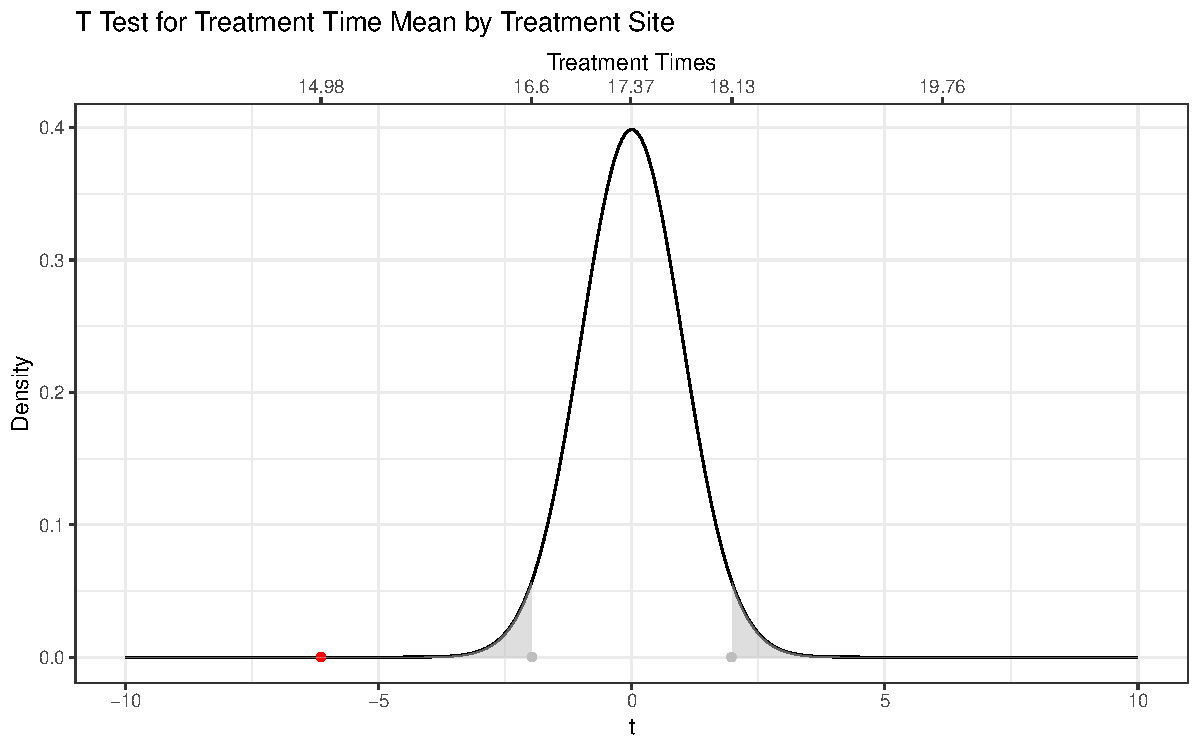
\includegraphics{HW2-045}
\newline
Our test statistic for this test is t = -6.138.
Our p-value is 0.0000. 0.0000 is < 0.05, meaning our test statistic is statistically significant and we reject the null. Our 95\% confidence interval is (-68.71283, -35.30646). This means that the true population mean for the difference in treatment time will fall between -68.71283 and -35.30646, 95\% of the time. The difference in means between the treatment sites is -13.61179. This does not fall within the confidence interval, meaning that we reject the null.
\newline
Failed Attempts:
\newline
\begin{Schunk}
\begin{Sinput}
> mu0<-mean(site.0$TIME)
> mu1<-mean(site.1$TIME)
> m <- mu1 - mu0
> n0<-length(site.0$TIME)
> n1<-length(site.1$TIME)
> alpha<-0.05
> se.xbar0<-sd(site.0$TIME)/sqrt(n0)
> se.xbar1<-sd(site.1$TIME)/sqrt(n1)
> t.obs1<-(mu1-mu0)/se.xbar1 #test statistic
> p.value<-pnorm(abs(t.obs)) #p value
> #tstat
> (mean(site.1$TIME)-mu0)/(sd(site.1$TIME/sqrt(length(site.1$TIME))))
> #check
> t.test(x=site.0$TIME, conf.level = 0.95, mu = m, var.equal = FALSE)
> t.test(x=site.1$TIME, conf.level = 0.95, mu = m, var.equal = FALSE)
\end{Sinput}
\end{Schunk}
  \end{enumerate}

%%%%%%%%%%%%%%%%%%%%%%%%%%%%%%%%%%%%%%%%%%%%%%%%%%%%%%%%%%%%%%%%%%%%%%%%%%%%%%%
%%%%%%%%%%%%%%%%%%%%%%%%%%%%%%%%%%%%%%%%%%%%%%%%%%%%%%%%%%%%%%%%%%%%%%%%%%%%%%%
%%%%%%%%%  END!
%%%%%%%%%%%%%%%%%%%%%%%%%%%%%%%%%%%%%%%%%%%%%%%%%%%%%%%%%%%%%%%%%%%%%%%%%%%%%%%
%%%%%%%%%%%%%%%%%%%%%%%%%%%%%%%%%%%%%%%%%%%%%%%%%%%%%%%%%%%%%%%%%%%%%%%%%%%%%%%
\end{enumerate}
\newpage
\bibliography{bib}
\end{document}
